% Created 2016-04-25 Mon 17:55
\documentclass[11pt]{article}
\usepackage[utf8]{inputenc}
\usepackage[T1]{fontenc}
\usepackage{fixltx2e}
\usepackage{graphicx}
\usepackage{grffile}
\usepackage{longtable}
\usepackage{wrapfig}
\usepackage{rotating}
\usepackage[normalem]{ulem}
\usepackage{amsmath}
\usepackage{textcomp}
\usepackage{amssymb}
\usepackage{capt-of}
\usepackage{hyperref}
\usepackage[portuguese, ]{babel}
\author{André Peric Tavares, Giulio Parva Denardi}
\date{\today}
\title{Projeto de Compiladores\\\medskip
\large Trabalho para a disciplina Compiladores na Universidade Federal do ABC sob orientação da Profa. Mirtha Lina Fernández Venero}
\hypersetup{
 pdfauthor={André Peric Tavares, Giulio Parva Denardi},
 pdftitle={Projeto de Compiladores},
 pdfkeywords={},
 pdfsubject={},
 pdfcreator={Emacs 24.5.1 (Org mode 8.3.3)}, 
 pdflang={Pt-Br}}
\begin{document}

\maketitle
\tableofcontents


\section{Introdução}
\label{sec:orgheadline1}
\textbf{negrito}
\emph{itálico}
\href{https://google.com}{google}

imagem:
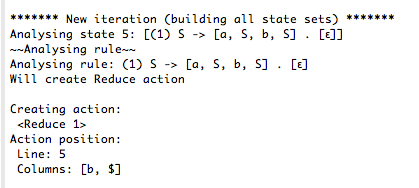
\includegraphics[width=.9\linewidth]{./media/Screenshot 2016-04-25 17.54.18.png}

\section{Objetivos}
\label{sec:orgheadline2}
\section{Justificativa}
\label{sec:orgheadline3}
\section{Metodologia de Projeto}
\label{sec:orgheadline4}
\section{Conclusão}
\label{sec:orgheadline5}
\section{Referências Bibliográficas}
\label{sec:orgheadline6}
\end{document}